\documentclass[a4paper,kul]{kulakarticle} %options: kul or kulak (default)

\usepackage[utf8]{inputenc}
\usepackage[dutch]{babel}
\usepackage{mhchem}

\usepackage{subcaption}
\usepackage{graphicx}



\date{Academiejaar 2018 -- 2019}	
\address{
  Master of Physics \\
  Visits to Research Laboratories in Belgium.  \\
  Prof. T. Cocolius}
\title{Visit of the Magnetometry Laboratory
	Report} 
\author{Jérôme Neirynck\\ Frederik Van Eecke\\ Robin Vrielynck\\ Robin Brambilla}

\begin{document}

\maketitle


\section{The cesium magnetometer.}
In order to make dipole measurements of the neutron possible a high resolution magnetic field sensor is necessary to fulfill the magnetic field stability requirement. The Cesium magnetometer used is based on the concept of optically detected magnetic resonance (ODMR) spectroscopy. Cesium is an alkali metal, which means there is one valence electron in an s-orbital. More specific the electronic configuration of cesium can be described as $[Xe]6s^{1}$.Therefore the interaction of Cesium with an external magnetic field is governed by the magnetic moment of its unpaired electron, aligned with the electron spin. Since the absorption of resonant polarized light also depends on the electron spin it is possible to link magnetic interactions via light dependent properties.\\ 

\paragraph{The cesium hyperfine and Zeeman structure}

The first step in understanding ODMR is a better understanding of the hyperfine and Zeeman structure in cesium. The only stable isotope of cesium is $\ce{^{133}_{55}Cs}$, which is used in all applications. It has a nuclear spin of $\frac{7}{2}.$ The interaction of this nuclear spin with the $J=\frac{1}{2}$ angular momentum provided by the valence electron results in a splitting of the ground state $6S_{\frac{1}{2}}$ into two hyperfine states $F = |I \pm J| = 3, 4$. These two hyperfine states are separated by an energy difference corresponding to a frequency of $9.2 GHz$. An energy scheme of $Cs$ is shown in figure \ref{fig:hyperfine}. The transition $D_{1}$ to the first excited state lies in the near-infrared (894.6 nm). The hyperfine interaction also splits this first excited state $6P_{\frac{1}{2}}$ into two hyperfine states corresponding with $f = 3,4$ separated by an energy difference corresponding to $1.2 GHz$. The zeeman splitting observed when an magnetic field is applied causes a further splitting of the hyperfine states into $2F+1$ degenerate sublevels, as shown in figure \ref{fig:zeeman}. More formal we say state $|F\rangle$ splits into $|F,m_{f}\rangle$ with $m_{f} = -F, -F+1,...,F-1,F$. The energy difference between those degenerate sublevels can be quantified with the Breit-Rabi\ref{eq: Breit-rabi} formula. Where $\mu_{b}$ is the Bohr magneton and $g_{f}$ is the Landé g-factor for the hyperfine level.
\begin{equation}
	\label{eq: Breit-rabi}
	\Delta E \left(M_{F}\right) = g_{f}\mu_{b}B_{0}M_{f} 
\end{equation}
From equation \ref{eq: Breit-rabi} it's easy to calculate the energy difference between two consecutive states and therefore the corresponding frequency, the Larmor frequency $\omega_{L}$. From equation \ref{eq: Larmor frequency} we get an expression for $\omega_{L}$, where $\gamma$ is the gyromagnetic ratio $\gamma = \frac{g_{f}\mu_{b}}{\hbar}$. Equation \ref{eq: Larmor frequency} is our first equation which relates a frequency to the applied magnetic field resulting in Zeeman splitting. From a very accurate knowledge of the gyromagnetic ratio, information concerning the magnetic field can be obtained resulting from frequency measurements. Which in physics is a very desired tool because frequency is the quantity which can be most precisely measured. In the cesium ground state $\gamma = 2\pi \cdot 3.5 Hz/nT$, a magnetic field in the order of $\mu T$ results in a (Larmor) frequency of some $kHz$, which can be measured very precisely.

\begin{equation}
	\label{eq: Larmor frequency}
	\omega_{L} = \frac{1}{\hbar}\left[\Delta E(M_{F+1} - \Delta E(M_{F}))\right] = \gamma B_{0}
\end{equation}

\begin{figure}[h!]
	\centering
	\begin{subfigure}{.5\textwidth}
		\centering
		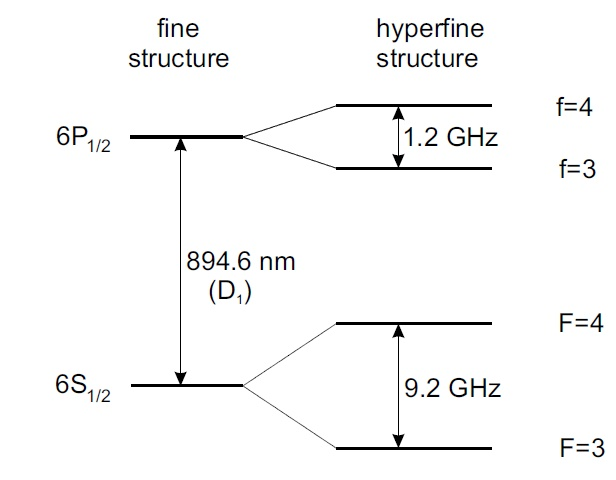
\includegraphics[width=.7\linewidth]{hyperfine}
		\caption{Energy scheme of $\ce{^{133}Cs}$. $D_{1}$ transition with hyperfine structure.}
		\label{fig:hyperfine}
	\end{subfigure}%
	\begin{subfigure}{.5\textwidth}
		\centering
		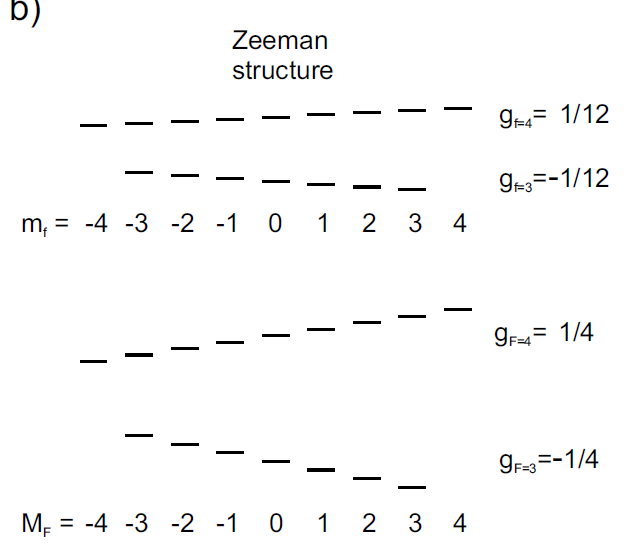
\includegraphics[width=.7\linewidth]{zeeman}
		\caption{Linear Zeeman effect in a small magnetic field (not to scale). The Zeeman levels presented are sublevels of the hyperfine levels presented in \ref{fig:hyperfine}  }
		\label{fig:zeeman}
	\end{subfigure}
\end{figure}

The general idea from which we want to determine the magnetic field is based on equation \ref{eq: Larmor frequency} and an exact knowledge of $\gamma$ for a certain transition. The component missing is an exact measurement of the energy difference and thereby the frequency between two neighboring Zeeman states. This magnetic resonance frequency will be determined using the optical properties linked with the spin state. To be able to use these optical properties it requires a preparation of our cesium gas done with the technique of optical pumping, which is discussed next.\\

\paragraph{Optical pumping}

The energy difference between the two ground state hyperfine levels is around $38 \mu eV$, which is smaller than the thermal energy at room temperature. The twp hyperfine states $F=4$ and $F=3$ are therefore equally populated. In order to observe magnetic resonance between Zeeman states a population imbalance is necessary. This imbalance is generated using optical pumping, which basically means you illuminate your sample which causes the transition to higher energy states. this can be done using a Cs discharge lamp with the disadvantage that their emission spectrum is very broad. As a consequence multiple possible transition are excited all at once. To avoid this we make us of a tunable laser which makes it possible to focus on the excitation of just one hyperfine transition. Moreover the laser has the advantage of providing a higher light intensity. In the literature consulted the laser is focused on the $D_{1}$ hyperfine transition: $6S_{\frac{1}{2}},F = 4 \rightarrow 6P_{\frac{1}{2}},f = 3$, as shown in figure \ref{fig:hyperfine}. We consider a laser producing right circularly polarized light $(\sigma^{+})$, this beam produced consist of photon carrying one unit of angular momentum. When absorbed by the atom the angular momentum of the atom increases by one. Mathematically speaking the laser excites transition from $|4,M\rangle$ states to $|3,M+1\rangle$ states. The atom is in an excited stated which spontaneously decays back into the ground state level, following the  selection rules $\Delta F = \pm1,0$ and $\Delta M = \pm1, 0$. The photon emitted during this decay can, because of the selection rules, posses an angular momentum of $0$ (linearly polarized) or $\pm 1$ (circularly polarized). The possible transitions induced by circularly polarized light and possible decay channels are shown on the left hand side of figure \ref{fig: transitions}.\\

During the absorption-emission pumping cycle an atom originally in a $|4,M\rangle$ state gets excited to an $|3,M+1\rangle$ state by absorption of a $\sigma^{+}$ photon. After decay following the selection rules the original $|4,M\rangle$ state can end up in a $|4,M\rangle$, $|4,M+1\rangle$ or $|4,M+2\rangle$ state. Depending on the angular momentum of the emitted photon. This means that a state cannot lose angular momentum during an absorption-emission single, but it can only earn angular momentum. When $\sigma^{+}$ light is applied to the sample the $F=4$ Zeeman level population is driven towards the $M = 3,4$ states. This result in the increase of population of those states as shown on the right hand side of figure \ref{fig: transitions}. These specific states cannot absorb $\sigma^{+}$ photons anymore and are called dark states. At this configuration out sample is completely polarized and the sample is completely transparent for $\sigma^{+}$ light. A major problem is the depolarization because of spin-exchange collisions and collisions whit the walls of the container.This depolarization because of collisions with the walls can be strongly reduced by coating the inner walls of the cell with paraffin. 




\begin{figure}[h!]
	\centering
	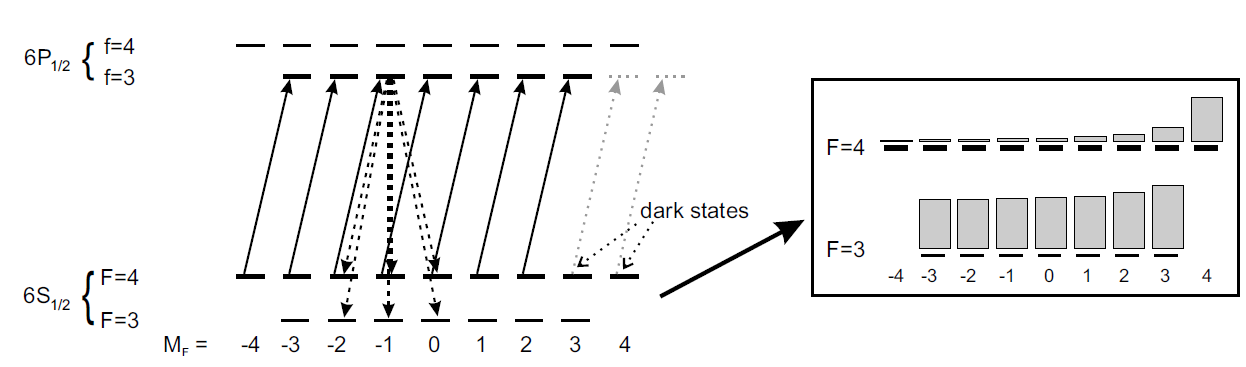
\includegraphics[width=\linewidth]{transitions}
	\caption{Transitions induced by right circularly polarized light are shown by the solid lines. The decay channels of the level $6P_{\frac{1}{2}} |f=3,m=-1\rangle$ are indicated by the dashed lines.}
	\label{fig: transitions}
\end{figure}

\paragraph{Optically detected magnetic resonance}	
When all atoms are in dark states and the sample is highly polarized, then our sample is highly polarized and transparent. At this point we reach a maximum in transmitted light intensity. We assume our sample is subject to a weak magnetic field $B_{0}$ resulting in a non degenerate Zeeman structure. By optical pumping with $\sigma^{+}$ light we assured all atoms are in dark states, which we can measure from the transmitted light intensity reaching a maximum. An additional applied resonance radio-frequency field can drive the transition between neighboring Zeeman states. Due to this r.f. field atoms escape from the dark states to states for which excitation by $\sigma^{+}$ is possible again. This results in a decrease in polarization because of the redistribution of spin states, which leads in the decrease of transmitted light intensity. Which we can measure. For one frequency for which a maximum change in transmitted light intensity is observed corresponds to $\omega_{L}$.\\

From measurements of the transmitted light intensity we are now able to determine the frequency corresponding with $\omega_{L}$. This information combined with the knowledge of the gyromagnetic ratio result through equation \ref{eq: Larmor frequency} in an exact value for $B_{0}$.  


\end{document}

